\begin{frame}[fragile]{Using UHD from Python (3/7)}

\footnotesize

\begin{itemize}
    \item \textbf{\textcolor{DarkBlue}{Step 3: Verify the UHD Python API}}
\end{itemize}

\hspace{2.8em}
\parbox{0.88\linewidth}{
\footnotesize
Verify that the UHD Python module is installed correctly by importing
the module, creating a USRP object, and configuring one of its parameters.
}

\vspace{0.2cm}

\scriptsize
\begin{Verbatim}[xleftmargin=3.8em]
>>> import uhd
>>> usrp = uhd.usrp.MultiUSRP("type=b200")
>>> usrp.set_rx_gain(70)
>>> print(usrp.get_rx_gain())
\end{Verbatim}

\vspace{0.3cm}

\begin{center}
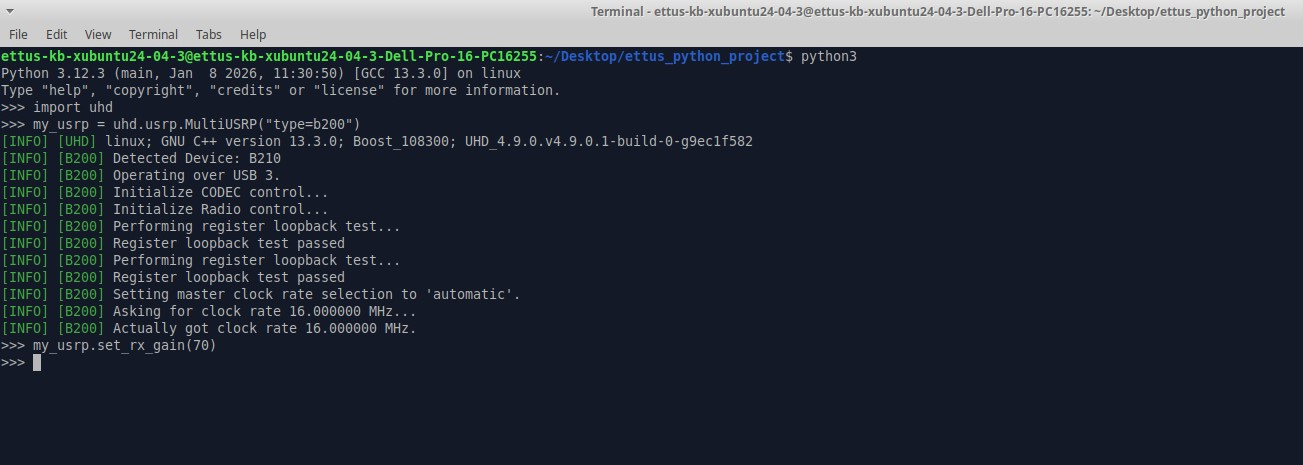
\includegraphics[width=0.88\linewidth,keepaspectratio]
{latex/jpg_png/image_python_api_basic importuhd_check B210.jpg}
\end{center}

\end{frame}